\section{What is artificial intelligence?}
\setauthor{Romeo Bhuiyan}

\section{Philosophy of artificial intelligence}
\setauthor{Christioph Lasinger}

\section{How does a neural network work?}
\setauthor{Romeo Bhuiyan}
A neural network is a type of machine learning algorithm modeled after the structure and function of a human brain (neural linking). It is composed of many interconnected processing nodes, called neurons, which work together to process information. 
\\
\\
Each neuron receives input from other neurons, processes that information, and produces an output. This output is then passed on to other neurons in the next layer of the network. In this way, information is passed through the network, from the input layer to the output layer, allowing the neural network to learn and make predictions based on the data it is given.
\\
\\
\\
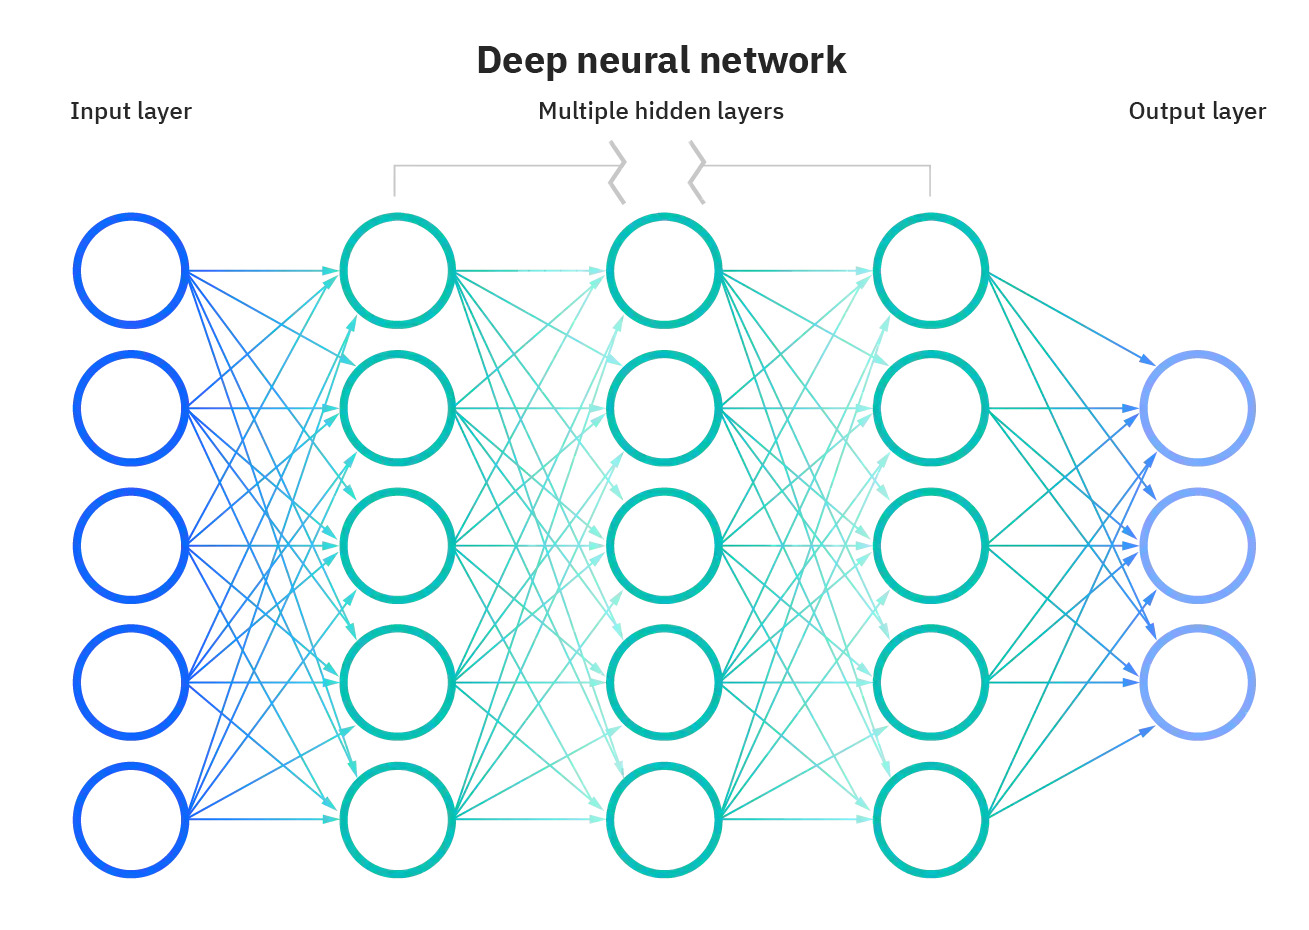
\includegraphics[width=1\textwidth]{pics/neuralnetwork.jpg}
\\
\\
\\
The specific details of how a neural network works can vary depending on its architecture and the type of problem it is being used to solve. But in general, a neural network is able to learn from data by adjusting the strength of the connections between its neurons, these connections being called weights, based on the input it receives. Over time, the network is able to improve its predictions by adjusting these weights in a way that minimizes errors between the network's output and the correct output.

\subsection{Solving Methods}
% Kommt noch

\section{How does face tracking work?}
\setauthor{Romeo Bhuiyan}
Face tracking is a technology that allows a computer or device to identify and monitor the movements of a person's face in real time. This is typically done using a combination of computer vision algorithms and specialized hardware, such as a camera or depth sensor.
\\
\\
To track a face, the system first detects the face in the video feed from the camera or depth sensor. This is typically done using a machine learning algorithm trained to recognize faces in images. Once the face has been detected, the system then uses various techniques to track the movements of the face, such as tracking the position of key facial features (such as the eyes and mouth) over time. This allows the system to accurately follow the face as it moves within the frame, even if it turns or changes orientation.
\\
\\
The resulting data can be used for a variety of purposes, such as enabling facial recognition (to identify who the person is), animating virtual characters, or controlling a user interface.

% Hier kommt noch eine Graphic hin von dem face tracking experiment von mediapipe mit python in anaconda
% maybe kann in die grafik eingegangen werden

\section{How does body tracking work?}
\setauthor{Romeo Bhuiyan}
Body tracking is the process of using technology to track the movement of a person's body. This is typically done using sensors or cameras that capture the movement of the body and then use algorithms to interpret that movement and translate it into digital data that can be used for various purposes. 
\\
\\
To track a body, the algorithm first detects the presence of a body in the video or data. It then uses various techniques to identify specific features of the body, such as the limbs, torso, or other distinctive features. This allows the algorithm to track the body as it moves over time. 
\\
\\
In addition to tracking the location of the body, some algorithms can also track other features, such as body movements or gestures. This allows them to be used for a variety of applications, such as video surveillance, virtual reality, gaming, human-computer interaction, and fitness tracking.

\section{The future of artificial intelligence}
\setauthor{Romeo Bhuiyan}
